
\chapter{Problemen tijdens het practicum.}\label{chap:apB}

In deze bijlage worden een aantal problemen omschreven die tijdens het practicum kunnen ontstaan.

\section{Adafruit\_Microbit.h: No such file or directory.}~\\
%Adafruit_Microbit.h: No such file or directory
%Adafruit\_Microbit.h: No such file or directory.\\
Contoleer of de Adafruit microbit geïnstalleerd is.
\begin{enumerate}
	\item Ga naar de library manager zoals aangegeven in figuur \ref{fig:ardLibMan}
	\item Controleer of library geinstalleerd is, zolas aangegeven in figuur \ref{fig:ardLibCon}
\end{enumerate}

\begin{figure}[h!]
	 		\centering
	  \begin{center} 	
		\begin{subfigure}[b]{0.45\textwidth}
     \includegraphics[width=0.7\textwidth]{figuren/arduinoManLib}
    \caption{selecteren van de library manager }
     \label{fig:ardLibMan}
   \end{subfigure}
\begin{subfigure}[b]{0.54\textwidth}
	     \includegraphics[width=0.98\textwidth]{figuren/arduinoManLibIns}
	\caption{Constrole Library is geïnstalleerd }
	\label{fig:ardLibCon}
\end{subfigure}
\captionsetup{justification=centering}
\caption{Controleren of library is geïnstalleerd. }
\label{fig:ardinopr1}
\end{center}

\end{figure}

\section{SerialPortException: Port name - COM..}~\\
java.io.IOException: jssc.SerialPortException: Port name - COM24; Method name - setEventsMask(); Exception type - Can't set mask.

De seriële poort is in gebruik door waarschijnlijk de monitor.

Sluit de monitor af.
 
 
\section{Tijdens het uploaden}
 Error: unable to find CMSIS-DAP device
 Error: No Valid JTAG Interface Configured.
 Error: No Valid JTAG Interface Configured.
 \begin{enumerate}
 	\item 
 Haal de USB stekker uit de laptop en doe deze opnieuw erin.
  \item Soms heeft het te maken met de firewall van windows.
  \begin{enumerate}
  	\item open Windows Defender Firewall.
  	\item Klik op: \texttt{\textit{Allow an app or feature through Windows Defender Firewall}}
   \item Klik op: Change settings.  	
   \item Zoek  naar \texttt{\textit{Arduino IDE}} en verwijder deze.  klik vervolgens op \texttt{\textit{OK}}.
   
   \item  Sluit de hele Arduino omgeven en start deze vervolgens weer op. De arduino zal vragen om toestemming, geef deze.
  \end{enumerate}
   \item Zelf uploaden van de code:
      \begin{enumerate}
            \item Zorg ervoor dat de hidden files zichtbaar worden. Ga met de File explorer naar de C: drive. klik op de . . . iets dergelijks als figuur \ref{fig:winOp} wordt zichtbaar klik op option en neem de optie show Hidden Files zoals figuur \ref{fig:hidFile} laat zien. 
            \begin{figure}[h!]
            	\centering
             		\begin{subfigure}[b]{0.49\textwidth}
            			\includegraphics[width=0.85\textwidth]{figuren/VerkennerOptions}
            			\caption{Selecteen van options bij de File Explorer }
            			\label{fig:winOp}
            		\end{subfigure}
            		\begin{subfigure}[b]{0.49\textwidth}
            			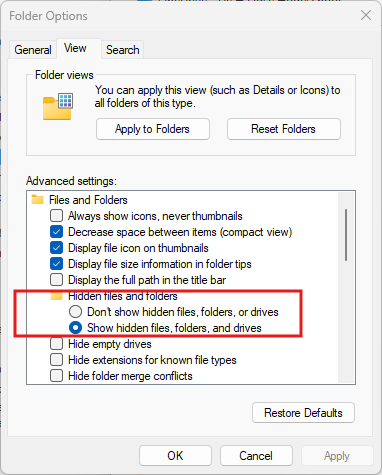
\includegraphics[width=0.7\textwidth]{figuren/windowsHiddenFile}
            			\caption{Maak hiddenfiles zichtbaar. }
            			\label{fig:hidFile}
            		\end{subfigure}
            		\captionsetup{justification=centering}
            		\caption{Hidden files zichtbaar maken }
            		\label{fig:hidF}
            	\end{figure}
            
   \item
       Compileer (Verify) \img{figuren/ardComp} je code. Arduino comipleert de file en maakt o.a. een \textbf{.hex} file aan. \\
          Deze \textbf{.hex} file moet gekopieerd worden naar de MICROBIT directory.\\
          Om de \textbf{.hex} file te vinden kan het beste naar het Output-veld van de \ardIDE ~gekeken worden.
          In één van de laatste regels in het Output-veld van de \ardIDE ~wordt de \textbf{.hex} file gecreëerd met het commando:\\
          \texttt{\textit{arm-none-eabi-objcopy -O ihex sourcefile\textbf{.elf} destinationfile\textbf{.hex}}}.\\ 
          In de destinationfile is het volledige pad te zien.\\
          In mijn geval staat er:\\
          \lstinline[stringstyle=\color{red}]| "C:\\Users\\john\\AppData\\Local\\Temp\\arduino\\sketches\\3490945EEE0644827B5A5400078BA5D3/blink.ino.hex"|\\
          Het hele pad in  mijn geval is dus:\\
           \lstinline[stringstyle=\color{red},basicstyle=\ttfamily\small]| "C:\Users\john\AppData\Local\Temp\arduino\sketches\3490945EEE0644827B5A5400078BA5D3"|\\
          \end{enumerate}       
  
 \end{enumerate}
 
 \section{Tijdens compileren  'kan stdint.h niet vinden'}
 Mogelijk is er iets fout gegaan bij het installeren van de \textbf{Add NRF5x Board Support}. Waardoor de library niet geinstalleed is.
 
 Bij het installeren van de 'Add NRF5x Board Support' moet er een lange tijd gewacht worden. Mogelijk is deze onderbroken. Bij het opnieuw installeren lijk alles goed te gaan, dit is echter niet zo.
 
 Mogelijke oplossing:\\
 remove het board en installeer deze opnieuw (wacht nu wel totdat deze geïnstalleerd is).
 
 